\documentclass{article}

\usepackage{amsmath, amsthm, amssymb, fancyhdr, graphicx}
\graphicspath{{./images/}}
\pagestyle{fancy}
\lhead{DREAL Paper Reading: MV-GPT}
\begin{document}
\paragraph{Abstract Summary:} Multimodal Video Generative Pretraining (MV-GPT) is this paper's
novel framework for learning from unlabelled videos which can effectively be used for generative
tasks such as multimodal video captioning.

\begin{itemize}
    \item Trains a multimodal video encoder and a sentence decoder jointly.
    \item Leverages future utterances as additional text sources, proposes a bidirectional
        generation objective --- generate future utterances given present multimodal context,
        and the present utterance given future observations.
    \item Train an encoder-decoder model end-to-end to generate a caption from raw pixels and
        transcribed speech directly.
\end{itemize}

\paragraph{Introduction:} A long-standing goal of AI is the development of conversational multimodal
systems that can both reliably perceive the world and effortlessly communicate with humans. 

\paragraph{}Multimodal video captioning tests both abilities; a successful model must not only accurately
understand \emph{'multimodal'} streams of input video (including speech and video frames), but also 
generate coherent natural language descriptions of the content.

\paragraph{Motivation:}In the field of computer vision and language learning, there is a lack of
large-scale, manually annotated data. Annotating captions for videos is time intensive, expensive,
and subjective (low inter-annotator agreement).

\paragraph{}This is largely in contrast with image classification, where fully annotated datasets are
orders of magnitude larger.

\paragraph{Pretraining:}One solution to this lack of data is the pretraining of video-language
models on instructional videos, in particular, domains where speech is particularly well aligned to 
visual content.

\paragraph{}Recent datasets of this nature include
\begin{itemize}
    \item Cooking312K
    \item HowTo100M
\end{itemize}

with associated captions from automatic speech recognition (ASR).

\paragraph{What is novel about this paper?}
\paragraph{}Contemporary models do not contain decoders, and lack the ability to generate
sentences. Only a video encoder is transferred to downstream tasks --- decoders are often
learned from scratch. 

\paragraph{}While one could initialize a decoder from independently pretrained weights such
as those from a GPT-2 model, the paper argues that this strategy is suboptimal, and performance
is significantly improved by optimizing the encoder and decoder jointly.

\paragraph{}Contemporary models attempt to solve this problem using a denoising autoencoder, wherein
the input speech to the model is artificially \emph{'noised'}, i.e. random words are masked out. Then the
decoder is tasked with reconstructing either the masked phrases or the original unmasked text. 

\paragraph{}In these frameworks, additional losses are often required to strengthen the pretraining
supervision, such as multimodal input alignment, and segment ordering.

\paragraph{}This paper's framework introduces a novel, stronger loss. It leverages future utterances as
an additional source of textual data, and trains a model to generate unseen sentences.


\begin{figure}

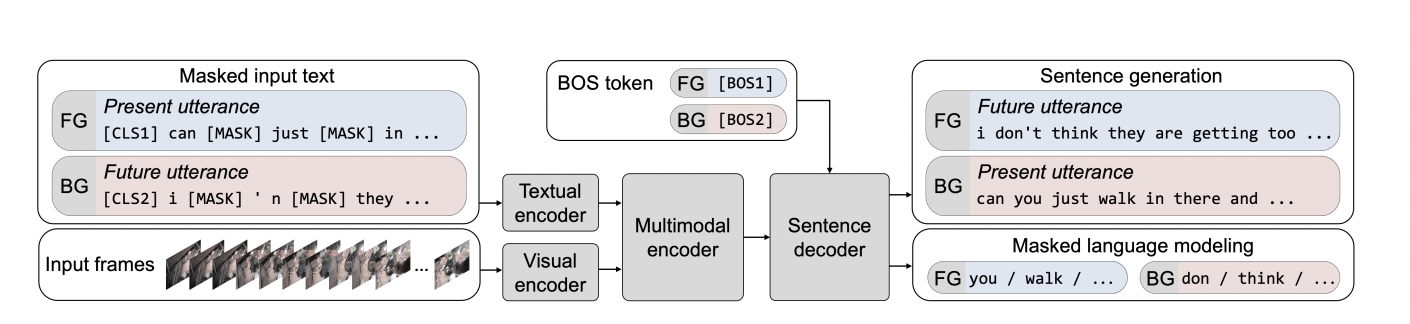
\includegraphics[width=11.6cm]{fig1}
\caption{Multimodal Video Generative Pretraining (MV-GPT) framework. \textbf{BG:} Backward generation, \textbf{FG:} Forward generation}



\end{figure}

\paragraph{}To alleviate the issue of future utterances being temporally unaligned, 
the paper proposes a backward generation objective, where present aligned utterances are 
generated given future utterances. 

\paragraph{}The paper's experimental results show that a model pretrained with this
bidirectional generation objective effectively transfers to multimodal video captioning
and largely outperforms the state of the art.

\paragraph{Method:} The paper's framework aims to take advantage of unlabelled instructional video data,
consisting of video frames and utterances often linked to the visual content.

\paragraph{}The framework requires two textual streams --- input to the encoder and a captioning target
for the decoder. Unlabelled videos do not have captioning targets, so they propose a simple
objective --- the model is trained to generate a \emph{future} utterance in the video given the current
video context and current utterances (forward generation). 

\paragraph{}This allows the model to learn how to optimally fuse modalities in the video encoder,
while the decoder is tasked with predicting a new utterance it has never seen before.

\paragraph{}The paper reiterates, however, that the goal is video captioning, and not "predicting
the future".

\paragraph{}To enable the model to generate text correspongind to the present video context, an
additional backward generation loss is added --- where the model must generate the current utterance given the 
current video frames and a future utterance (backward generation).

\paragraph{}This allows generated sentences to be temporally aligned (and hence more tightly coupled) with 
the visual inputs.

\paragraph{Bi-directional Utterance Generation}

\paragraph{}Given a large set of unlabelled videos, the authors extract short clips
consisting of visual frames $F = \{f_1 ,\ldots, f_{N_f}\}$ and transcribed speech utterances
$U = \{u_1, \ldots, u_{N_u}\}$ aligned with $F$.

\paragraph{}The immediate future utterance $W = \{w_1, \ldots, w_{N_w}\}$, is also considered,
where $u_i$, $w_j$ are the tokenized words in the transcribed utterances. 'Utterances' refer
to a single sentence of transcribed speech.

\paragraph{Forward Generation:} The model is trained to generate a future utterance $W$ given
clip frames $F$ and present utterances $U$. Formally speaking, the formulation for
the forward generation objective to minimize negative log-likelihood of the true future
utterance $W$, where loss given by the chain rule is 
\[
    L_{FG} = -\sum_{i=1}^{N_w} \log P(w_i | w_1,\ldots,w_{i-1}, F, U)
\]

\paragraph{Note:}The visual input $F$ is temporally aligned with the decoder output $U$. This loss
functions encourages the network to generate a caption related to the visual contents.

\paragraph{Backward Generation:} The model applies the same loss as forward generation, now in the 
backward direction. The model is tasked with generating present utterances $U$ aligned with video frames
$F$, conditioned on future utterances $W$ and $F$. Like in forward generation, the following negative
log-likelihood of true present utterance is minimized:

\[
    L_{BG} = -\sum_{i=1}^{N_u}log P(u_i | u_1,\ldots , u_{i-1}, F, W) 
\]

\paragraph{Note:}The visual input $F$ is temporally aligned with the decoder output $U$. This loss function
encourages the network to generate captions related to the visual contents.

\paragraph{Masked Language Modeling:} The model uses masked language modeling as an additional
supplementary loss $L_{MLM}(X)$, where $X$ is the input utterance on which the masking is applied.
This loss is applied on both the forward and backward input utterances, i.e. as 
$L_{MLM}(U)$ and $L_{MLM}(W)$. These losses are computed independently from the above bidirectional
generation losses. 

\paragraph{Model:} The MV-GPT model consists entirely of transformer blocks, and is trained
end-to-end directly from pixels and word tokens.

\paragraph{Modality Specific Encoders:}Given a multimodal video input consisting of the visual frames $F = \{f_1, \ldots, f_{N_f}\}$,
and text inputs $X = \{x_1, \ldots, x_{N_x}\}$, the model first extracts feature from the individual
modalities indepedently. The textual input $X$ is the aligned utterance $U$ in general (for computing
forward generation loss and for downstream captioning tasks) but is set to $W$ when computing the
backward generation loss.
\paragraph{Textual Encoder:}$N_x$ textual embeddings, $E = \{e_i\}$, are extracted from the input
text using a BERT encoder.
\paragraph{Visual Encoder:}Visual features are extracted directly from pixels, using the transformer-based
encoder ViViT.
\end{document}
